
\section{Raspberry Pi}
\label{sec:Raspberry-Pi}

Após constatado que o ESP8266 não oferece modo promíscuo, foi testado e
desenvolvido software para transformar o Raspberry Pi em uma plataforma para
hospedar o sensor. Sua principal diferença é o sistema operacional linux
(inexistente no ESP8266) que favorece o Raspberry e o alto custo que o
desfavorece. Em média no exterior o Raspberry Pi é vendido por USD \$ 35,00
\cite{RPI2016} e no Brasil entre R\$ 270 em Março de 2016 e R\$ 190 em Janeiro
de 2017 \cite{rpi3-mercadolivre}.

As vantagens de ter um computador moderno completo sobrepõem seu custo em muitas
vezes, dentre as quais destacamos a interface "amigável" com usuário devido ao
sistema operacional oferecendo maior nível de abstração (bastando apenas alguns
comandos para acessá-los realizar tarefas complexas) e o poder computacional.
Além deste recurso a nível de sistema, a comunidade e número de projetos "faça
você mesmo" é muito maior que a do ESP8266, devido a sua simplicidade em
conectar-se a um monitor e construir protótipos e aplicações.

O RPI3 (\emph{Raspberry PI 3 Model B}) é um computador \emph{single-board}  (única
placa) que tem o tamanho próximo ao de um cartão de crédito. Foi desenvolvido
pela \emph{Raspberry Pi Foundation} para promover o ensino da computação nas
escolas. Este computador possui:


\begin{alineas}
	\item 1 GB RAM;

	\item Processador Gráfico \emph{VideoCore IV 3D};

	\item ARM CPU de 1.2 GHz quad-core 64-bit.

	\item 4 portas USB;

	\item 40 pinos GPIOs;

	\item Porta HDMI;

	\item Porta \emph{Megabit Ethernet};

	\item Saída de aúdio e vídeo 3.5 mm;

	\item Interface para câmera (CSI) e monitor (DSI);

	\item Leitor para cartão \emph{micro SD};

	\item \emph{Wi-Fi LAN} embutida 802.11n;

	\item \emph{Bluetooth 4.1} e \emph{Bluetooth Low Energy} (BLE);

\end{alineas}

\begin{figure}[htb]
	\caption{\label{fig:rpi-3}Raspiberry Pi 3 }
	\begin{center}
		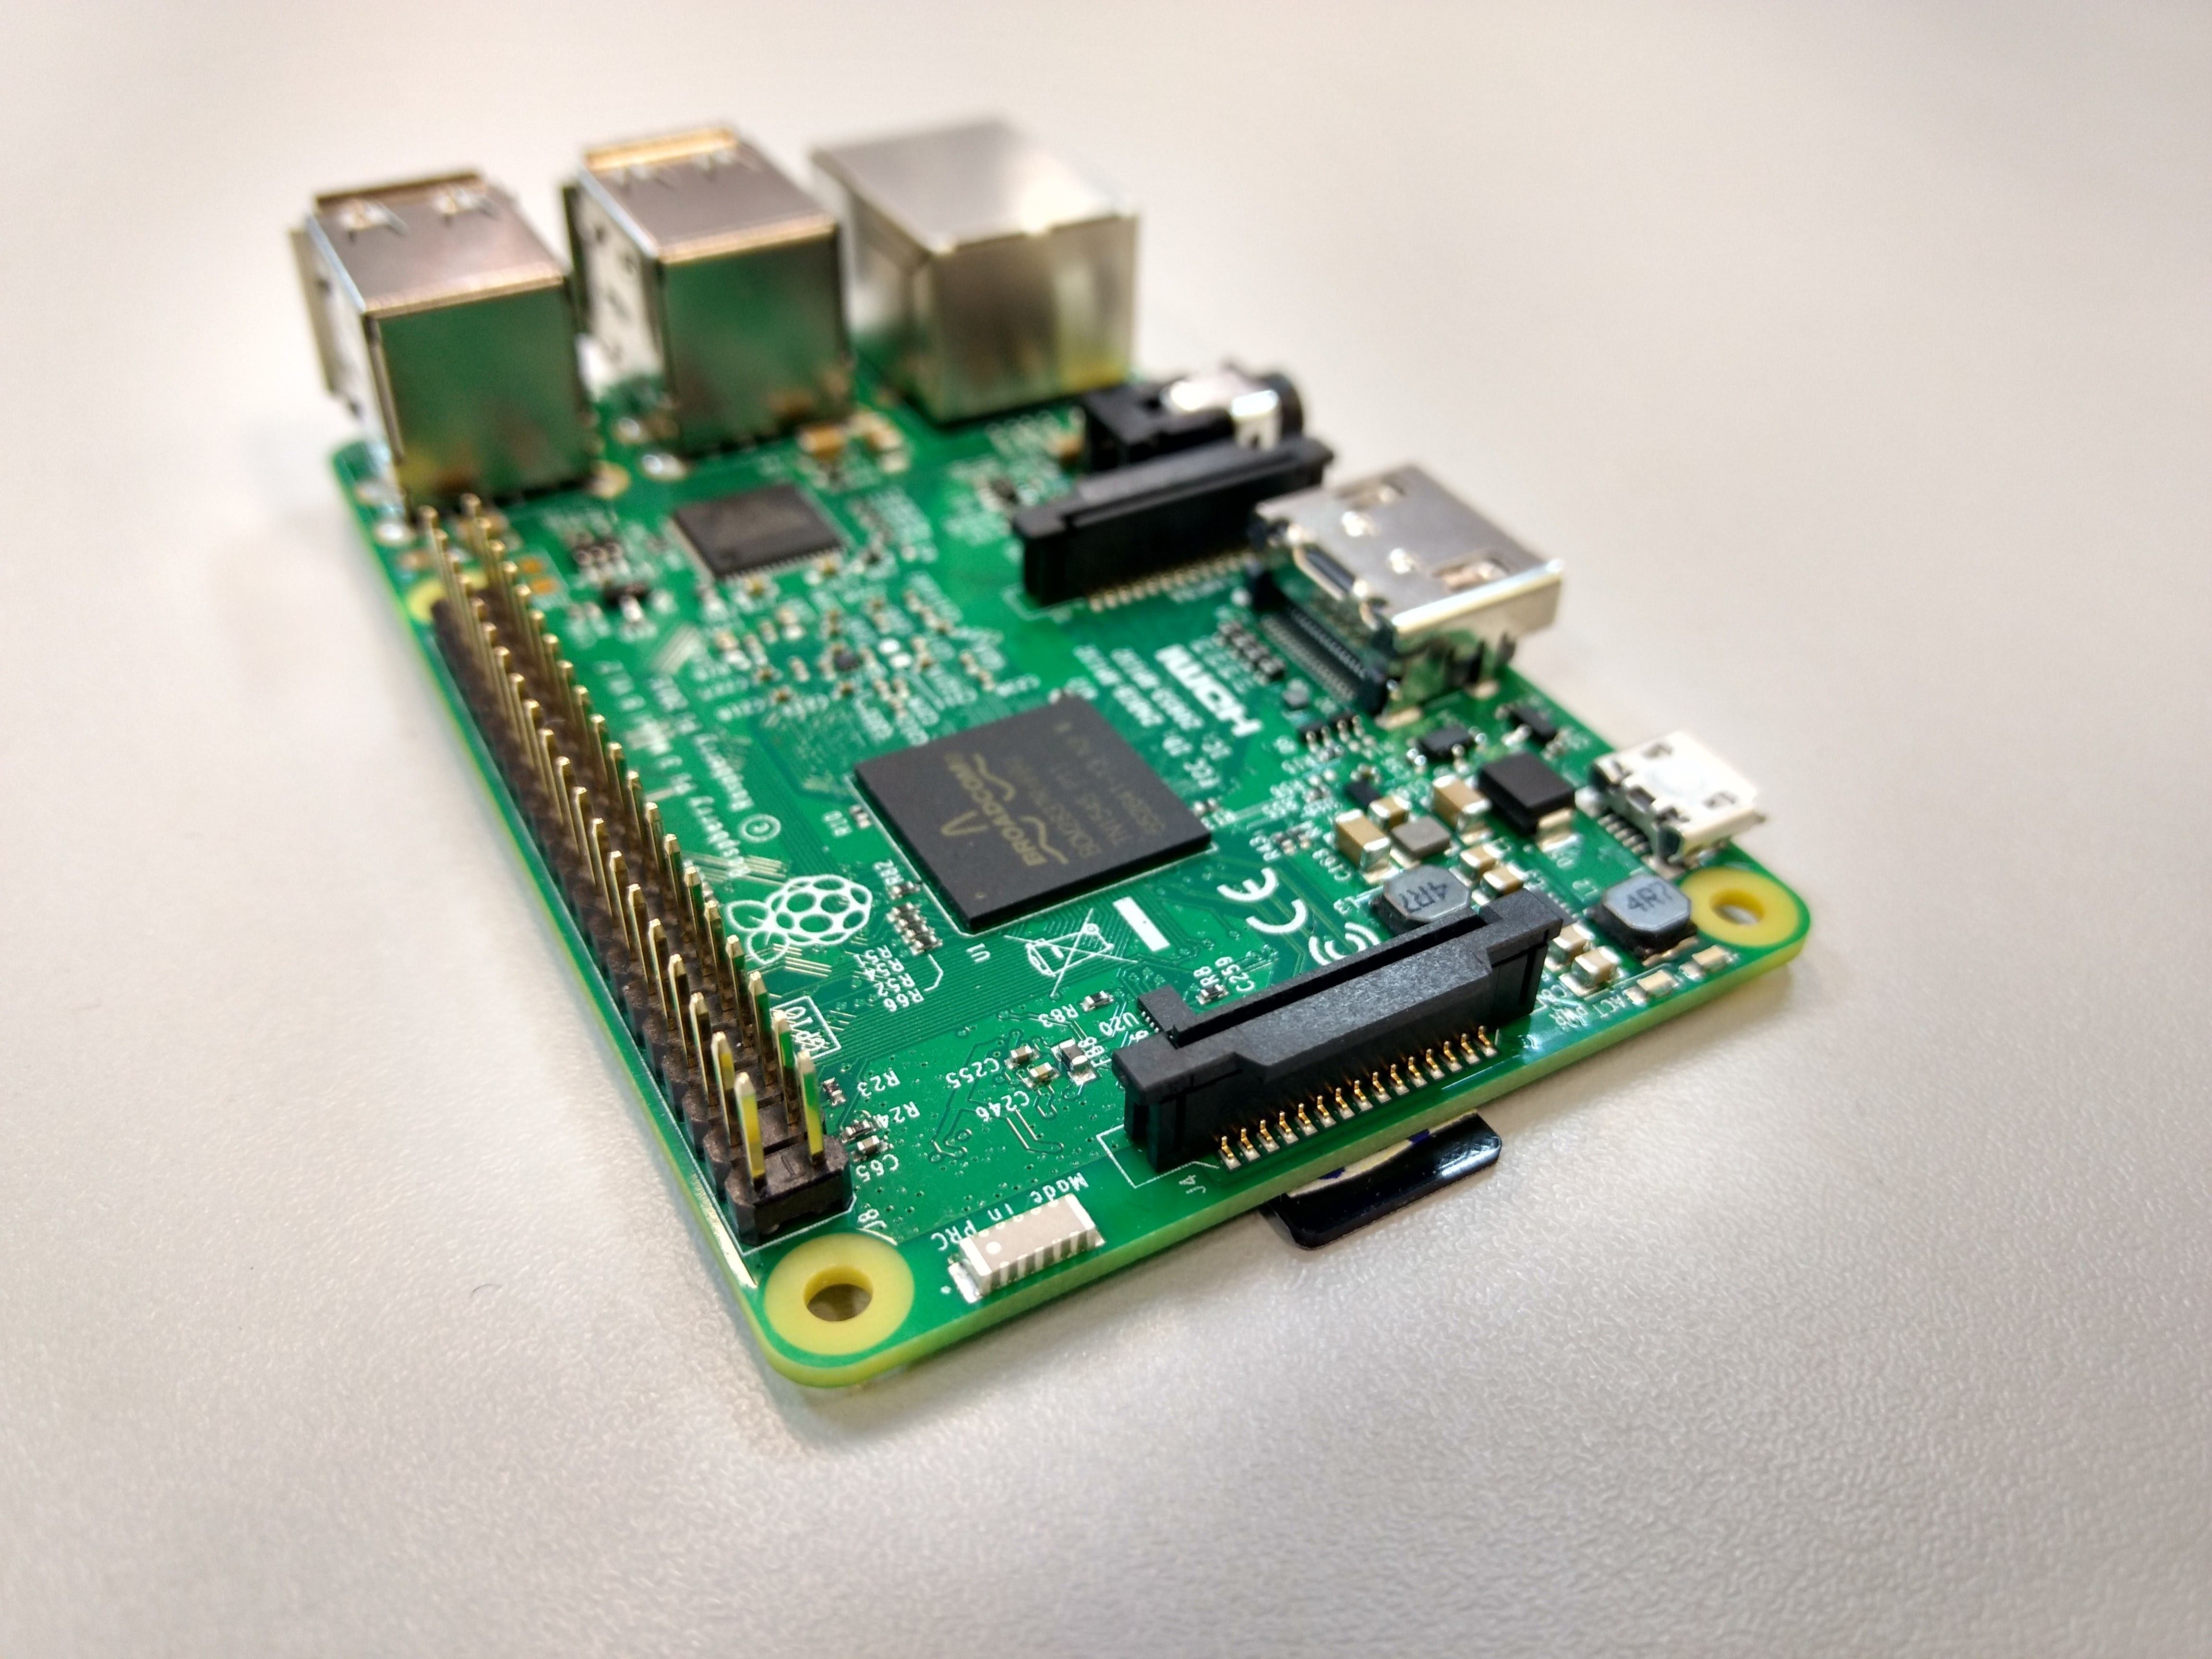
\includegraphics[width=1\textwidth]{040-plataformas/RPi-Wi-Fi-dongles/rpi-onboard.jpg}
	\end{center}
	\legend{Fonte: Elaborada pelo autor}
\end{figure}



\subsection{Disponibilidade no mercado}
\label{subsec:mercado-esp}

Para abordar a disponibilidade no mercado devemos também contar os periféricos
que são necessários para desenvolver na plataforma  RPI3 da mesma maneira que
foi feito com o ESP8266.

O RPI3 é ligado por uma fonte de 2A, 5V e 10W através de uma entrada micro
USB. Para ligá-la, foi adquirido uma fonte USB tipo A para iPad, pois além de
poder desconectar o cabo da fonte, facilitando a manutenção, fornece a
quantidade exata de amperagem que o computador precisa. A primeira aquisição foi
de um carregador de \emph{smartphone} que não forneceu os amperes necessários.

Em comparação com a anterior, esta geração  tem uma exigência energética maior,
muito disto é devido a \emph{Wi-Fi} integrado que é um destaque desta geração.
A antena de cerâmica do adaptador integrado pode ser vista no primeiro plano da
\selfref{fig:rpi-3}. Contudo, o adaptador não possui modo promíscuo e fez-se
necessário o uso de adaptadores \emph{Wi-Fi} USB. As recomendações da comunidade
quanto a escolha do adaptador USB (também conhecido como \emph{dongle Wi-Fi})
são o \emph{Edimax EW-7811Un} que não é tão comum no Brasil e o
\emph{EDUP EP-N85xx} que tem muitos genéricos no mercado nacional.

Como camada de \emph{software} o RPI3 comporta diversos sistemas operacionais que são carregados de seu
cartão \emph{microSD}. Alguns exemplos de sistemas compatíveis são
\emph{Archlinux}, \emph{OpenELECE}, \emph{Raspbian}, \emph{Risc OS},
\emph{Pidora}, \emph{Kali Linux}, \emph{Windows 10 IoT}, entre outros. Para este
trabalho, foi utilizado o \emph{Raspbian} cuja interface é mostrada na
\selfref{fig:raspbian-jessie}.

\begin{figure}[htb]
	\caption{\label{fig:raspbian-jessie}Raspbian Jessie com Pixel}
	\begin{center}
		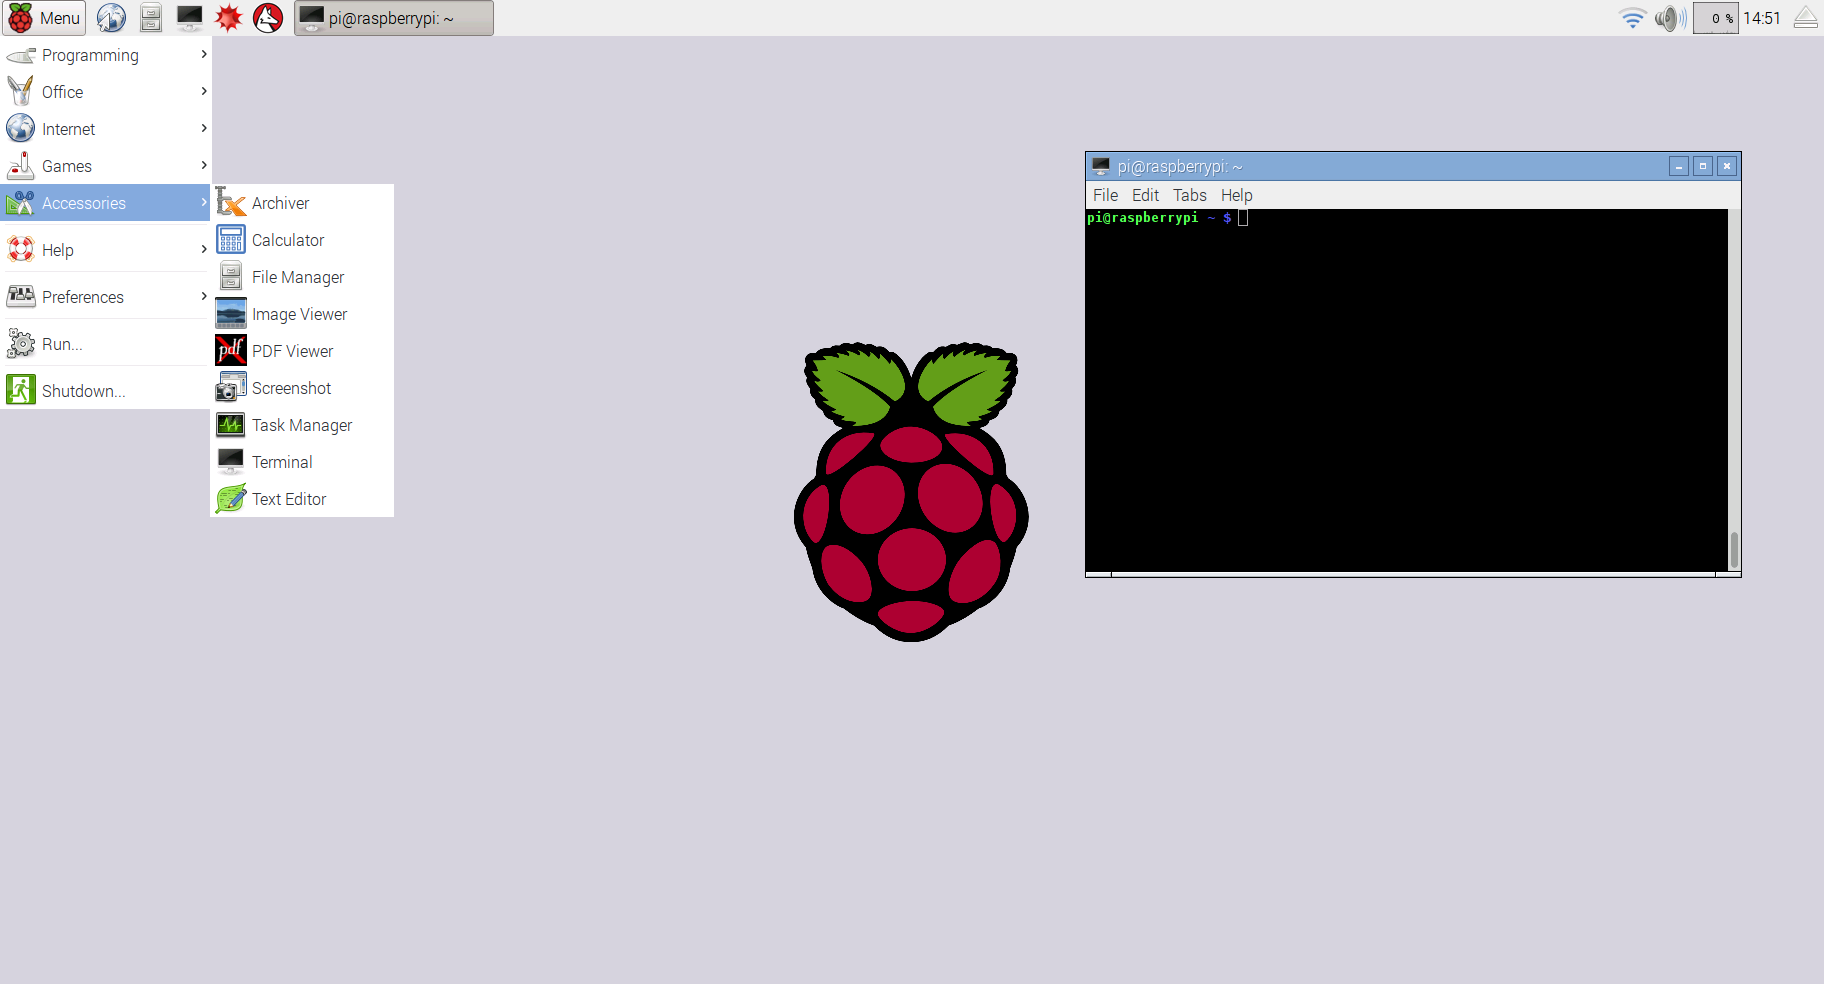
\includegraphics[width=1\textwidth]{040-plataformas/RPi-Wi-Fi-dongles/raspbian.jpg}
	\end{center}
	\legend{Fonte: Elaborada pelo autor}
\end{figure}

Portanto Para funcionamento e desenvolvimento de aplicações com RPI3 são
necessários componentes extra que são  demonstrados na
\selfref{table:custo-rpi}.

\begin{table}[htb]
\IBGEtab{%
\ABNTEXchapterfont {
	\caption{Descrição e custos com Raspberry Pi 3}%
	\label{table:custo-rpi}
}
}{%
\begin{tabular}{ccc}
\toprule
Produto								&	Descrição e utilização					&	Custo		\\
\midrule \midrule
Novo Raspberry Pi 3 (pi3)			&											&			 	\\
Quadcore 1.2ghz (10x+rapido) 1gb	&	Computador hospedeiro do sensor			&	R\$ 269,99	\\
\midrule
Fonte Carregador Original Usb		&	Fonte com conector USB tipo A que		&				\\
Apple Iphone 3 4 4s Ipad 1 2		&	supriu o consumo elétrico do RPI3		&	R\$ 13,99	\\
\midrule
Cabo USB com conectores 			&											&				\\
\emph{A} e \emph{Micro-B} 			&	Para conectar a fonte ao RPI3			&	R\$ 2,00^{1}	\\
\midrule
Cartão Micro Sdhc 16gb Ultra Sd 	&	Armazena o SO e outros arquivos, a		&				\\
Sandisk Classe 10 30mb/s			&	classe indica a velocidade do cartão	&				\\
									&	que implica na velocidade do SO			&	R\$ 21,99	\\
\midrule
Mini Adaptador Wireless Wifi 		&	Adaptador externo Wi-Fi que  			&				\\
Edup Usb 150mbps Raspberry Pi		&	permite modo promíscuo					&	R\$ 16,88	\\
\midrule
\bottomrule
\end{tabular}%
}{%
	\fonte{Produzido pelo autor.}%
	\nota[Nota 1]{Os cabos USB foram reutilizados de outras aplicações.}%
}
\end{table}

\subsection{Testes e resultados}
\label{subsec:mercado-esp}

De maneira análoga à feita com o ESP8266 analisamos a capacidade do Raspberry Pi
de  operar com sua wi-fi em modo promíscuo porém, diferentes ferramentas foram
utilizadas  devido  a diferença de camada de software envolvida. Neste caso
utilizamos as ferramentas airodump e tshark além das ferramentas de Wi-Fi
padrões do sistema operacional raspbian.

\begin{verbatim}
	sudo ifconfig wlan0 down
	sudo iwconfig wlan0 mode monitor
\end{verbatim}

Para verificar o modo  promíscuo no ambiente raspbian utiliza-se os comandos iw
que são padrão do sistema operacional Debian.  como   Este comando foi realizado
teste  utilizando somente o adaptador  de wi-fi integrado   no rpi.  o resultado
foi negativo portanto  outros adaptadores foram necessários.

No ambiente do laboratório encontramos adaptadores wi-fi USB d-link Porém
executando o mesmo teste neles não foi possível Ativar o modo promíscuo.  Com
colega podemos emprestar um terceiro adaptador,  este do modelo ePub

Para capturar e avaliar pacotes É necessário uma ferramenta  para tal. Na área
de segurança da informação podemos encontrar Aero Jump que é utilizado para
Avaliar explorar vulnerabilidades de segurança em rede sem fio.  Outra área que
forneceu uma ferramenta adequada é a área de qualidade de serviço em redes de
computadores onde o software wireshark é bem popular,  uma interface alternativa
do mesmo  feita para uso em terminal é chamada tShark.


**Conclusão sobre Raspberry Pi**

O Raspberry foi adotado como o sensor para detectar os dispositivos. O modo
promíscuo conseguiu ser acessado através de adaptador/módulo USB Wi-Fi. Mais
detalhes sobre a construção e adoção deste computador serão apresentados no
capítulo "Construção".

**Comparativo RPi X ESP8266**

Em comparação com o ESP8266, o Raspberry Pi compensou seu custo mais caro devido
a facilidade de programação e acesso aos seus recursos e integração e acesso a
recursos externos. Além disso, foi possível chegar ao modo promíscuo facilmente
através do Bash e do sistema operacional. A seguir, uma tabela comparando as
principais características do RPi e do módulo ESP12F.

\begin{figure}[htb]
	\caption{\label{fig:raspbian-jessie}Raspbian Jessie com Pixel}
	\begin{center}
		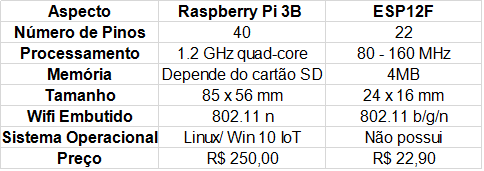
\includegraphics[width=1\textwidth]{040-plataformas/Plataformas DIY e comparacao/rpi-esp.png}
	\end{center}
	\legend{Fonte: Elaborada pelo autor}
\end{figure}
